% !TeX program = xelatex
% !TeX encoding = UTF-8
% !TeX TXS-program:compile = txs:///xelatex | txs:///xelatex
\documentclass[aspectratio=169, table, 12pt]{beamer}

% Preamble bersama seluruh slide mata kuliah ini.
% Dipanggil dari slides/sessionXX/sessionXX.tex tepat sesudah baris
% \documentclass[aspectratio=169, table, 12pt]{beamer}
% Paket tambahan yang hanya dibutuhkan satu sesi ditulis di berkas sesi itu.

\usepackage{colortbl}
\usepackage{xcolor}
\usepackage{listings}
\usepackage{tabularx}
\usepackage{booktabs}
\usepackage{tikz}
\usepackage{pgfplots}
\usepackage{fontspec}
\usepackage[english,bahasai]{babel}
\pgfplotsset{compat=1.18}
\usetikzlibrary{arrows.meta, positioning, calc, fit, shapes.geometric,
  shapes.multipart, backgrounds, matrix, chains, trees}

\makeatletter
\def\input@path{{../theme/}}
\makeatother
\graphicspath{{../theme/}{../../figures/}}
% Stub symlink Windows memakai tema cadangan sampai aset institusi tersedia.
\IfFileExists{../theme/beamerthemePradita.sty}{%
  \usetheme{Pradita}
}{%
  \usetheme{Madrid}
  \setmainfont{TeX Gyre Heros}
  \setsansfont{TeX Gyre Heros}
  \setbeamertemplate{navigation symbols}{}
}

\definecolor{praditagreen}{RGB}{37, 113, 71}
\setbeamercolor{structure}{fg=praditagreen}
\setbeamercolor{palette primary}{bg=praditagreen,fg=white}
\setbeamercolor{palette secondary}{bg=praditagreen!80!black,fg=white}
\setbeamercolor{palette tertiary}{bg=praditagreen!60!black,fg=white}
\setbeamerfont{frametitle}{size=\large}
\setbeamertemplate{caption}[numbered]

% Ukuran header mengikuti teks agar judul panjang tidak menabrak logo.
\setbeamercolor{frametitle}{bg=white,fg=black}
\setbeamertemplate{frametitle}{%
  \begin{beamercolorbox}[wd=\paperwidth,sep=0.2cm]{frametitle}
    \begin{minipage}[c]{0.77\paperwidth}
      \raggedright\fontsize{16}{18}\selectfont\bfseries\insertframetitle
      \ifx\insertframesubtitle\empty\else
        \par\small\mdseries\insertframesubtitle
      \fi
    \end{minipage}\hfill
    \begin{minipage}[c]{0.15\paperwidth}
      \IfFileExists{../theme/classFiles/logo_universitas.png}{%
        
\includegraphics[width=\linewidth]{../theme/classFiles/logo_universitas.png}%
      }{}
    \end{minipage}
  \end{beamercolorbox}
}
\setbeamertemplate{footline}{%
  \ifnum\value{framenumber}>1
    \begin{beamercolorbox}[wd=\paperwidth,ht=0.35cm,dp=0.15cm,
      leftskip=0.3cm,rightskip=0.3cm]{palette primary}
      \footnotesize\bfseries\insertframenumber/\inserttotalframenumber
      \hfill IT40513
    \end{beamercolorbox}
  \fi
}
\DeclareRobustCommand{\berkas}[1]{\path{#1}}

% Tema membuat garis tabel berwarna putih. Dikembalikan agar tabel terbaca.
\arrayrulecolor{black}
\setlength{\arrayrulewidth}{0.5pt}

\lstdefinelanguage{yaml}{
  basicstyle=\ttfamily\scriptsize,
  keywordstyle=\color{blue}\bfseries,
  commentstyle=\color{gray}\itshape,
  stringstyle=\color{red},
  showstringspaces=false,
  breaklines=true,
  frame=lines,
  numbers=none,
  backgroundcolor=\color{lightgray!10},
  tabsize=2,
  morecomment=[l]{\#}
}

\lstdefinelanguage{json}{
  basicstyle=\ttfamily\scriptsize,
  stringstyle=\color{red},
  commentstyle=\color{gray},
  breaklines=true,
  showstringspaces=false,
  tabsize=2,
  numbers=none,
  frame=lines,
  backgroundcolor=\color{lightgray!10},
  string=[s]{"}{"}
}

\lstdefinelanguage{bash}{
  keywords={},
  basicstyle=\ttfamily\scriptsize,
  ndkeywords={docker, kubectl, helm, curl, git, terraform},
  ndkeywordstyle=\color{purple}\bfseries,
  sensitive=true,
  commentstyle=\color{gray},
  numbers=none,
  breaklines=true,
  frame=lines,
  backgroundcolor=\color{lightgray!10},
  tabsize=2,
  comment=[l]{\#},
  showstringspaces=false
}

\lstdefinelanguage{http}{
  keywords={GET, POST, PUT, PATCH, DELETE, HEAD, OPTIONS, HTTP},
  basicstyle=\ttfamily\scriptsize,
  keywordstyle=\color{blue}\bfseries,
  sensitive=true,
  numbers=none,
  breaklines=true,
  frame=lines,
  backgroundcolor=\color{lightgray!10},
  tabsize=2,
  showstringspaces=false
}

\subtitle{IT40513 · Enterprise Architecture \& Digital Blueprint}
\author{\textbf{Alfa Yohannis}}


% Sampul membatasi judul di panel putih tema rujukan Pradita.
\setbeamertemplate{title page}{%
  \begin{tikzpicture}[remember picture,overlay]
    \node[anchor=north west,inner sep=0pt,text width=8.8cm]
      at ([xshift=1cm,yshift=-3.15cm]current page.north west) {%
        {\small\insertsubtitle\par}\vspace{0.25cm}
        \resizebox{8.8cm}{!}{\begin{minipage}{12cm}
          \raggedright\color{praditagreen}\bfseries\inserttitle
        \end{minipage}}
      };
    \node[anchor=south west,inner sep=0pt]
      at ([xshift=1cm,yshift=1.65cm]current page.south west)
      {\small\insertdate};
    \node[anchor=west,inner sep=0pt,text=white]
      at ([xshift=0.8cm,yshift=0.75cm]current page.south west)
      {\small\insertauthor};
  \end{tikzpicture}
}


% Batasi kedua dimensi gambar agar diagram bersama tetap berada pada slide.
\newsavebox{\eafigbox}
\newcommand{\eadiagram}[1]{%
  \sbox{\eafigbox}{\resizebox{0.94\textwidth}{!}{\input{#1}}}%
  \ifdim\dimexpr\ht\eafigbox+\dp\eafigbox\relax>0.64\textheight
    \resizebox{!}{0.64\textheight}{\usebox{\eafigbox}}%
  \else
    \usebox{\eafigbox}%
  \fi
}


\title{\Huge Orientasi dan Dasar\\ \vspace{10pt} Arsitektur Enterprise}
\date{Pertemuan 01}

\begin{document}

\frame{\titlepage}

\begin{frame}
  \frametitle{Isi Pertemuan}
  \vspace{14pt}
  \begin{columns}[t]
    \column{0.5\textwidth}
    {\small\tableofcontents[sections={1-3}]}

    \column{0.5\textwidth}
    {\small\tableofcontents[sections={4-5}]}
  \end{columns}
\end{frame}

\begin{frame}{\hfill}
  \centering
  \Huge{\textbf{Siapa yang memegang\\peta besar organisasi?}}
\end{frame}

\section{Tujuan dan Konteks}

\begin{frame}{\hfill}
  \centering
  \Huge{\textbf{Tujuan dan Konteks}}
\end{frame}

\begin{frame}{{\Large Tujuan Pembelajaran}}
  \vspace{10pt}
  \begin{itemize}
    \item Menjelaskan masalah organisasi yang dijawab EA (\textit{Enterprise Architecture}) dan nilai
          yang dapat diharapkan darinya, dengan merujuk bukti empiris.
    \item Mendeskripsikan sebuah organisasi memakai lima sudut pandang bersama: strategi, bisnis,
          data, aplikasi, dan teknologi.
    \item Menyusun piagam tim dan profil organisasi sebagai titik awal \textit{capstone}.
  \end{itemize}
\end{frame}

\begin{frame}{{\Large Diagram Konsep Bab 1}}
  \centering
  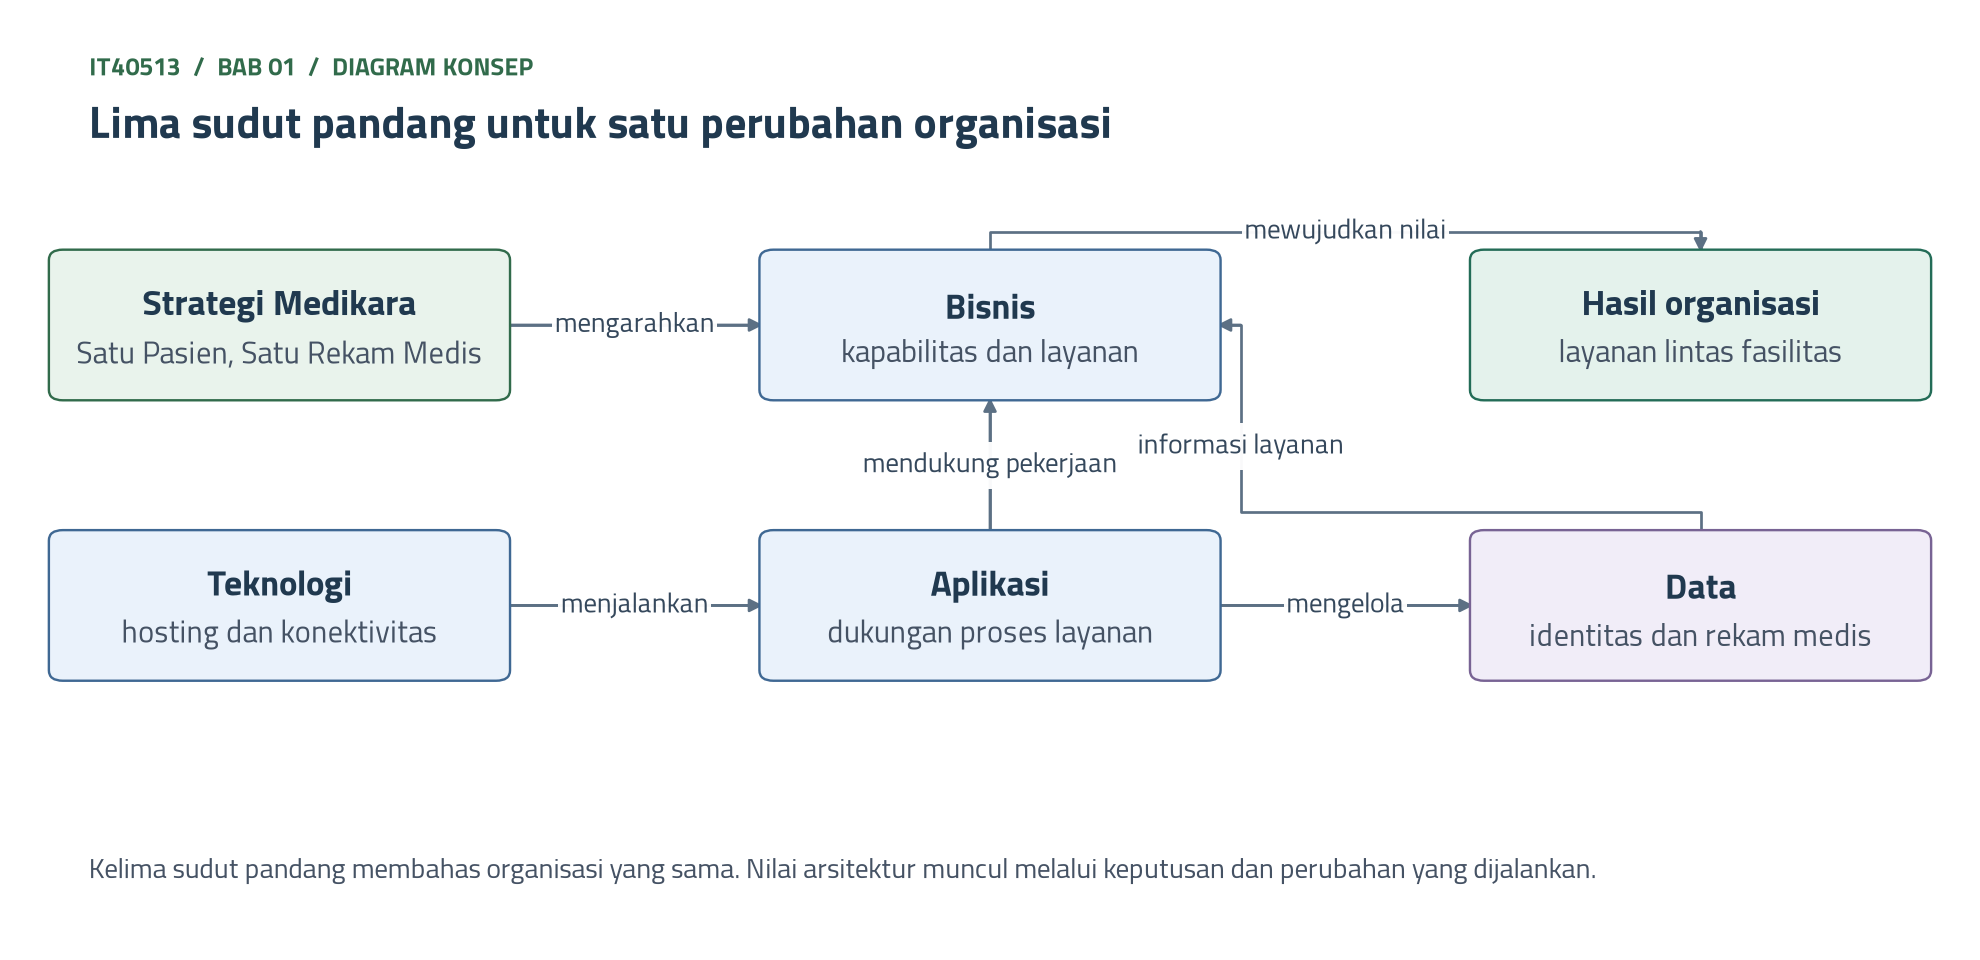
\includegraphics[width=0.96\textwidth,height=0.77\textheight,keepaspectratio]{../../figures/ch01-diagram-konsep.png}
  \label{fig:session01-ilustrasi-bab}
\end{frame}

\section{Enterprise dan Arsitektur}

\begin{frame}{\hfill}
  \centering
  \Huge{\textbf{Enterprise dan\\Arsitektur}}
\end{frame}

\begin{frame}{{\Large Empat Gejala Tanpa Arsitektur}}
  \vspace{10pt}
  \begin{itemize}
    \item Sistem ganda: dua aplikasi atau lebih mengerjakan fungsi yang sama di unit berbeda.
    \item Data tersebar: satu pelanggan tercatat di beberapa sistem dengan isi yang tidak sama.
    \item Integrasi menumpuk: setiap sistem baru disambungkan sendiri-sendiri.
    \item Keputusan tanpa gambaran utuh: proyek disetujui satu per satu.
    \item Penyebabnya bukan orang yang ceroboh, melainkan tidak ada yang bertugas menjaga gambaran
          utuh.
  \end{itemize}
\end{frame}

\begin{frame}{{\Large Enterprise, Arsitektur, dan EA}}
  \vspace{6pt}
  \small
  \begin{itemize}
    \item \textit{Enterprise}: tingkat tertinggi deskripsi organisasi menurut TOGAF. Batasnya
          ditentukan tujuan bersama, bukan akta pendirian.
    \item Arsitektur menurut ISO/IEC/IEEE 42010:2022: konsep atau sifat mendasar suatu entitas di
          dalam lingkungannya, beserta prinsip yang mengatur perwujudan dan perubahannya.
    \item TOGAF dan ISO sama-sama memuat tiga unsur: bagian, hubungan, dan prinsip.
    \item Arsitektur berbeda dari deskripsinya: setiap organisasi sudah punya arsitektur, entah
          dirancang atau terbentuk secara kebetulan.
    \item EA: praktik berkelanjutan untuk memahami \textit{enterprise} secara utuh, dari strategi
          sampai teknologi, lalu mengarahkan perubahan.
  \end{itemize}
\end{frame}

\begin{frame}{{\Large EA Adalah Praktik, Bukan Dokumen}}
  \vspace{6pt}
  \small
  \begin{itemize}
    \item Dokumen dan diagram adalah alat kerja. Hasil yang dicari adalah keputusan yang lebih baik.
    \item Kotusev: artefak EA menjembatani komunikasi pemangku kepentingan bisnis dan TI (Teknologi
          Informasi).
    \item Analogi: rencana tata ruang kota memuat zona, jalan utama, dan aturan, bukan setiap rumah.
    \item Misalkan distributor dengan 9 gudang cabang punya empat aplikasi stok: laporan nasional
          dirakit dua staf selama empat hari kerja tiap akhir bulan.
    \item Misalkan bank daerah membeli aplikasi pinjaman digital: proyek Rp3,5 miliar tertunda
          sembilan bulan demi penghubung yang tidak dianggarkan.
  \end{itemize}
\end{frame}

\begin{frame}{{\Large Tiga Arsitektur yang Sering Tertukar}}
  \scriptsize
  \begin{tabularx}{\textwidth}{>{\raggedright\arraybackslash}p{1.9cm}
      >{\raggedright\arraybackslash}X >{\raggedright\arraybackslash}X
      >{\raggedright\arraybackslash}X}
    \hline
    \textbf{Aspek} & \textbf{EA} & \textbf{Arsitektur solusi} & \textbf{Arsitektur perangkat lunak} \\
    \hline
    Cakupan & Seluruh \textit{enterprise} & Satu inisiatif atau satu layanan & Satu sistem perangkat lunak \\
    \hline
    Pertanyaan utama & Apa yang diubah lebih dahulu, dan mengapa? & Bagaimana inisiatif ini dibangun dari sistem yang ada? & Bagaimana sistem ini disusun di dalamnya? \\
    \hline
    Horizon & Beberapa tahun, misalnya 2026 sampai 2030 & Selama proyek berjalan & Selama umur sistem \\
    \hline
    Pembaca utama & Direksi, pimpinan unit, arsitek lain & Sponsor, manajer proyek, vendor & Tim pengembang dan tim operasi \\
    \hline
    Contoh luaran & Prinsip, \textit{capability map}, peta jalan & Rancangan solusi satu proyek & Diagram komponen, keputusan desain \\
    \hline
    Padanan tata kota & Rencana tata ruang kota & Rancangan satu kawasan perumahan & Gambar kerja satu rumah \\
    \hline
  \end{tabularx}

  \vspace{6pt}
  \small Kesalahan paling sering: salah tingkat, misalnya diagram komponen satu aplikasi dibawa ke
  rapat direksi.
\end{frame}

\begin{frame}{{\Large Lanskap Sistem Medikara Saat Ini}}
  \centering
  \eadiagram{../../figures/ch01-lanskap-medikara.tex}
\end{frame}

\begin{frame}{{\Large Kasus: Lima Rumah Sakit, Lima SIMRS}}
  \begin{block}{Kasus Medikara Health}
    \small
    \begin{itemize}
      \item Sistem ganda: lima SIMRS (Sistem Informasi Manajemen Rumah Sakit) mengerjakan fungsi yang
            sama.
      \item Data tersebar: misalkan pasien dirawat di Bekasi lalu berobat di Depok. Ia punya dua nomor
            rekam medis, dan riwayat alerginya tidak terlihat di Depok.
      \item Integrasi menumpuk: $5 \times 4 = 20$ sambungan dipelihara terpisah. Perubahan aturan klaim
            BPJS Kesehatan dikerjakan lima kali.
      \item Keputusan tanpa gambaran utuh: laporan manajemen dirakit lewat \textit{spreadsheet}.
      \item Pemegang peta besar belum ada. Tim \textit{capstone} berlatih mengisi posisi itu.
    \end{itemize}
  \end{block}
\end{frame}

\section{Sudut Pandang dan Istilah}

\begin{frame}{\hfill}
  \centering
  \Huge{\textbf{Sudut Pandang\\dan Istilah}}
\end{frame}

\begin{frame}{{\Large Antrean 50 Menit, Tiga Jawaban}}
  \vspace{10pt}
  \begin{itemize}
    \item Misalkan direksi bertanya mengapa antrean pendaftaran rawat jalan mencapai 50 menit.
    \item Kepala layanan: petugas loket kurang.
    \item Kepala TI: server pendaftaran lambat setiap pagi.
    \item Bagian keuangan: verifikasi kepesertaan BPJS Kesehatan memakan waktu.
    \item Tanpa cara bersama untuk melihat organisasi, rapat berakhir dengan tiga proyek terpisah.
  \end{itemize}
\end{frame}

\begin{frame}{{\Large Lima Sudut Pandang atas Organisasi}}
  \centering
  \eadiagram{../../figures/ch01-lima-sudut-pandang.tex}
\end{frame}

\begin{frame}{{\Large Perubahan Merambat Dua Arah}}
  \vspace{6pt}
  \small
  \begin{itemize}
    \item Turun dari strategi: misalkan jaringan klinik bekerja sama dengan 6 klinik mitra. Satu
          keputusan menghasilkan empat pekerjaan pada bisnis, data, aplikasi, dan teknologi.
    \item Naik dari teknologi: misalkan server SIMRS tidak lagi didukung pabrikannya mulai tahun depan.
          Target antrean tahun itu terancam.
    \item Analogi: denah, gambar listrik, pipa air, dan jalur gas medis satu gedung. Ruang operasi
          pindah, gambar lain wajib ikut berubah.
    \item Bagi direksi, kelima sudut pandang diringkas menjadi satu halaman sebagai alat bicara.
    \item Ross, Weill, dan Robertson menyebutnya \textit{core diagram}. Bab 3 membahasnya.
  \end{itemize}
\end{frame}

\begin{frame}{{\Large Kasus: Satu Kunjungan Rawat Jalan}}
  \begin{block}{Kasus Medikara Health}
    \scriptsize
    \begin{tabularx}{\linewidth}{>{\raggedright\arraybackslash}p{1.5cm}
        >{\raggedright\arraybackslash}X >{\raggedright\arraybackslash}X}
      \hline
      \textbf{Sudut pandang} & \textbf{Yang terlihat di Medikara Depok} & \textbf{Masalah yang muncul} \\
      \hline
      Strategi & Sasaran ``Satu Pasien, Satu Rekam Medis'' dan antrean lebih pendek & Belum ada ukuran waktu tunggu yang sama di kelima rumah sakit \\
      \hline
      Bisnis & Janji temu, pendaftaran, verifikasi BPJS, pemeriksaan, resep, obat & Pasien yang sudah janji temu tetap mendaftar ulang di loket \\
      \hline
      Data & Identitas pasien, kunjungan, catatan dokter, resep, klaim & Identitas di Medikara+ dan SIMRS Depok dicocokkan manual \\
      \hline
      Aplikasi & Medikara+, SIMRS Depok, sambungan BPJS Kesehatan dan SATUSEHAT & Data janji temu diketik ulang ke SIMRS \\
      \hline
      Teknologi & Server SIMRS di Depok, jaringan ke server vendor Medikara+ & Server melambat pada jam sibuk pagi \\
      \hline
    \end{tabularx}

    \vspace{4pt}
    Menambah petugas loket hanya menyentuh baris bisnis. Antrean kembali panjang begitu jumlah
    pasien naik.
  \end{block}
\end{frame}

\begin{frame}{{\Large Satu Kata, Banyak Arti}}
  \vspace{6pt}
  \small
  \begin{itemize}
    \item Misalkan rapat menyepakati sistem baru ``harus terintegrasi dengan SIMRS''. Kepala layanan
          membayangkan data seketika, tim TI berencana mengirim berkas tiap malam.
    \item Glosarium bersama memuat istilah, arti yang disepakati, contoh pemakaian, istilah yang
          sering dikira sama, dan pemilik istilah.
    \item Analogi: daftar singkatan resmi rumah sakit mencegah salah obat.
    \item ``Selesai'': misalkan selisih tiga bulan kerja tambahan senilai Rp600 juta, di luar kontrak.
    \item ``Biaya aplikasi'': misalkan tim TI melaporkan Rp200 juta, sedangkan bagian keuangan
          menghitung total lima tahun Rp1,4 miliar.
  \end{itemize}
\end{frame}

\begin{frame}{{\Large Istilah Teknis dan Analoginya}}
  \scriptsize
  \begin{tabularx}{\textwidth}{>{\raggedright\arraybackslash}p{1.8cm}
      >{\raggedright\arraybackslash}X >{\raggedright\arraybackslash}X}
    \hline
    \textbf{Istilah} & \textbf{Arti singkat} & \textbf{Analogi} \\
    \hline
    Aplikasi & Program yang membantu satu pekerjaan, misalnya pendaftaran pasien & Formulir dan buku catatan petugas dalam bentuk digital \\
    \hline
    Basis data & Tempat aplikasi menyimpan data secara tertata agar mudah dicari dan diperbarui & Lemari arsip dengan map berlabel \\
    \hline
    Server & Komputer yang menjalankan aplikasi untuk banyak pengguna sekaligus & Dapur warung yang melayani semua meja \\
    \hline
    Integrasi & Cara dua aplikasi bertukar data, seketika atau berkala & Kurir antarkantor: ada yang tiap jam, ada yang tiap malam \\
    \hline
    API & Pintu resmi aplikasi untuk menerima permintaan dari aplikasi lain dengan format yang disepakati & Loket dengan formulir baku: permintaan lewat loket, tidak masuk ke gudang \\
    \hline
    \textit{On-premise} & Server dimiliki dan dirawat sendiri di gedung organisasi & Memiliki dan merawat genset sendiri \\
    \hline
    \textit{Cloud} & Daya komputasi disewa dari penyedia lewat jaringan, sesuai pemakaian & Berlangganan listrik tanpa merawat pembangkitnya \\
    \hline
  \end{tabularx}
\end{frame}

\begin{frame}{{\Large Istilah Bisnis dan Pertanyaannya}}
  \scriptsize
  \begin{tabularx}{\textwidth}{>{\raggedright\arraybackslash}p{1.8cm}
      >{\raggedright\arraybackslash}X >{\raggedright\arraybackslash}X}
    \hline
    \textbf{Istilah} & \textbf{Arti singkat} & \textbf{Pertanyaan yang dijawab} \\
    \hline
    Strategi & Pilihan arah jangka menengah: di mana bersaing dan bagaimana menang & Apa yang dikerjakan, dan apa yang sengaja tidak dikerjakan? \\
    \hline
    Model bisnis & Cara organisasi menciptakan, menyerahkan, dan menangkap nilai & Dari mana pendapatan datang, dan untuk nilai apa? \\
    \hline
    Model operasi & Tingkat integrasi dan standardisasi proses bisnis untuk melayani pelanggan & Proses dan data mana yang harus sama di semua unit? \\
    \hline
    Biaya modal dan operasional & Belanja sekali di awal lawan belanja berulang tiap periode & Berapa dibayar sekarang, berapa tiap tahun? \\
    \hline
    Nilai & Manfaat yang dirasakan dibandingkan pengorbanannya & Apa yang menjadi lebih baik, dan bagi siapa? \\
    \hline
    \textit{Stakeholder} & Pihak yang punya kepentingan atas sebuah sistem atau perubahan & Siapa diuntungkan atau dirugikan, dan apa kekhawatirannya? \\
    \hline
  \end{tabularx}
\end{frame}

\section{Nilai EA dan Peran Arsitek}

\begin{frame}{\hfill}
  \centering
  \Huge{\textbf{Nilai EA dan\\Peran Arsitek}}
\end{frame}

\begin{frame}{{\Large Apa yang Didapat dari Rp1,8 Miliar?}}
  \vspace{10pt}
  \begin{itemize}
    \item Misalkan usulan tim arsitektur tiga orang berbiaya Rp1,8 miliar per tahun.
    \item ``Gambaran utuh organisasi'' tidak tercatat di laporan laba rugi.
    \item Tamm dkk.: EA tidak menghasilkan manfaat secara langsung.
    \item Manfaat mengalir lewat empat pemungkin (\textit{benefit enablers}).
    \item Analogi: resep tidak menyembuhkan. Pasien sembuh bila resepnya ditebus dan obatnya diminum.
  \end{itemize}
\end{frame}

\begin{frame}{{\Large Manfaat Mengalir Lewat Empat Pemungkin}}
  \centering
  \eadiagram{../../figures/ch01-mekanisme-nilai.tex}
\end{frame}

\begin{frame}{{\Large Dua Pemungkin, Dua Hitungan}}
  \vspace{6pt}
  \small
  \begin{itemize}
    \item Optimalisasi portofolio: misalkan tiga aplikasi penjadwalan dokter, masing-masing Rp150 juta
          per tahun.
    \item Menyatukannya menghemat $2 \times$ Rp150 juta = Rp300 juta per tahun, belum dikurangi biaya
          peralihan.
    \item Ketersediaan informasi: misalkan laporan kunjungan bulanan disusun dua staf selama 6 hari
          kerja, lalu turun menjadi 1 hari kerja.
    \item Penghematannya 5 hari $\times$ 2 staf = 10 hari kerja per bulan, atau 120 hari kerja per
          tahun.
    \item Penghematan muncul karena katalog dipakai dalam keputusan anggaran, bukan karena katalognya
          ada.
  \end{itemize}
\end{frame}

\begin{frame}{{\Large Empat Faktor Keberhasilan Lange dkk.}}
  \scriptsize
  \begin{tabularx}{\textwidth}{>{\raggedright\arraybackslash}p{2.1cm}
      >{\raggedright\arraybackslash}X >{\raggedright\arraybackslash}X}
    \hline
    \textbf{Faktor} & \textbf{Artinya} & \textbf{Pertanyaan pemeriksaan} \\
    \hline
    Mutu produk & Artefak EA benar, mutakhir, dan sesuai kebutuhan pembacanya & Apakah artefak terakhir dipakai dalam satu keputusan selama tiga bulan terakhir? \\
    \hline
    Mutu infrastruktur & Alat, repositori, dan cara kerja yang membuat artefak mudah dibuat dan dicari & Dapatkah manajer proyek menemukan katalog aplikasi tanpa bertanya ke arsitek? \\
    \hline
    Mutu layanan & Dukungan arsitek kepada proyek dan unit bisnis, tepat waktu dan berguna & Berapa hari yang dibutuhkan untuk meninjau satu usulan proyek? \\
    \hline
    Penambatan organisasi & EA melekat pada anggaran, persetujuan proyek, dan tata kelola & Apakah persetujuan proyek mensyaratkan tinjauan arsitektur? \\
    \hline
  \end{tabularx}

  \vspace{6pt}
  \small Survei 133 praktisi. Penambatan organisasi menjadi pusat model. Kepuasan pengguna tidak
  terbukti berguna untuk menentukan maupun mengukur keberhasilan EA.
\end{frame}

\begin{frame}{{\Large Survei SAP LeanIX: Dibaca Kritis}}
  \vspace{6pt}
  \small
  \begin{itemize}
    \item EA Insights 2025, 360 arsitek: 92 persen menyatakan EA dipandang, seluruhnya atau sebagian,
          sebagai fungsi administratif TI.
    \item 51 persen organisasi membutuhkan sebulan atau lebih untuk satu keputusan arsitektur.
    \item Hanya 15 persen menyertakan wakil seluruh lini bisnis dalam dewan peninjau arsitektur.
    \item Hanya 14 persen responden menyatakan EA dipandang sebagai mitra dekat bisnis.
    \item Respondennya arsitek di organisasi pelanggan SAP LeanIX, penjual alat EA, sehingga sampelnya
          tidak mewakili seluruh organisasi.
  \end{itemize}
\end{frame}

\begin{frame}{{\Large Lima Penyebab Kegagalan Praktik EA}}
  \scriptsize
  \begin{tabularx}{\textwidth}{>{\raggedright\arraybackslash}p{3.3cm}
      >{\raggedright\arraybackslash}X >{\raggedright\arraybackslash}X}
    \hline
    \textbf{Penyebab} & \textbf{Gejala} & \textbf{Penawar} \\
    \hline
    EA terpisah dari pengelolaan TI & Tim arsitektur dan proyek berjalan sendiri-sendiri & Tinjauan arsitektur ditambatkan pada persetujuan anggaran dan proyek \\
    \hline
    Dokumentasi jarang dipakai & Model besar tidak pernah dibuka lagi & Artefak dibuat atas permintaan pembaca untuk keputusan tertentu \\
    \hline
    Arsitek tanpa kewenangan & Prinsip dilanggar tanpa akibat & Mandat tertulis dari direksi dan alur dispensasi (Bab 14) \\
    \hline
    Mengejar model lengkap lebih dahulu & Berbulan-bulan memotret kondisi saat ini tanpa manfaat & Mulai dari keputusan yang mendesak, model diperluas secukupnya \\
    \hline
    EA dipandang urusan TI & Tidak ada wakil bisnis dalam peninjauan & Pimpinan unit bisnis menjadi pemilik artefak bisnis \\
    \hline
  \end{tabularx}

  \vspace{6pt}
  \small \textit{Capability map} tidak perlu memuat 300 kapabilitas bila keputusan yang dihadapi hanya
  menyangkut 20 di antaranya.
\end{frame}

\begin{frame}{{\Large Peran Arsitek Enterprise}}
  \small
  \begin{itemize}
    \item Kotusev: praktik EA terdiri atas perencanaan strategis, pelaksanaan inisiatif, dan
          optimalisasi teknologi yang berjalan bersamaan.
    \item Tugas: memelihara gambaran kondisi saat ini, menyusun prinsip dan peta jalan, serta meninjau
          usulan proyek.
    \item Analogi: juru bahasa tidak memutuskan isi perjanjian, tetapi memastikan kedua pihak memahami
          hal yang sama.
    \item Misalkan sistem antrean daring Rp900 juta menyimpan identitas sendiri. Syarat arsitek:
          memakai identitas dari SIMRS, biaya integrasi bertambah Rp120 juta.
    \item Misalkan usulan pembaruan server total Rp2,4 miliar. Direksi memilih memperpanjang
          pemeliharaan Rp450 juta.
  \end{itemize}
\end{frame}

\begin{frame}{{\Large Arsitek dan Pihak di Sekitarnya}}
  \scriptsize
  \begin{tabularx}{\textwidth}{>{\raggedright\arraybackslash}p{2.4cm}
      >{\raggedright\arraybackslash}X >{\raggedright\arraybackslash}X}
    \hline
    \textbf{Pihak} & \textbf{Yang diberikan arsitek} & \textbf{Yang dibutuhkan arsitek} \\
    \hline
    Direksi & Pilihan investasi beserta akibat dan \textit{tradeoff}-nya, dalam satu halaman & Arah strategi, prioritas, dan mandat \\
    \hline
    Pimpinan unit bisnis & Kepastian bahwa kebutuhan unitnya masuk peta jalan & Penjelasan proses, masalah, dan ukuran keberhasilan \\
    \hline
    Manajer proyek & Batasan arsitektur yang jelas sejak awal proyek & Rancangan solusi untuk ditinjau dan jadwal keputusan \\
    \hline
    Tim TI dan vendor & Standar, prinsip, dan antarmuka yang disepakati & Informasi teknis tentang produk, batasan, dan biaya \\
    \hline
  \end{tabularx}

  \vspace{6pt}
  \small Manajer proyek menjaga lingkup, jadwal, dan biaya satu proyek. Arsitek menjaga kecocokan
  proyek itu dengan keseluruhan. Direksi memutuskan investasi, arsitek menyiapkan pilihan beserta
  akibatnya.
\end{frame}

\section{Capstone, Aktivitas, dan Latihan}

\begin{frame}{\hfill}
  \centering
  \Huge{\textbf{Capstone, Aktivitas,\\dan Latihan}}
\end{frame}

\begin{frame}{{\Large Empat Mata Kuliah, Satu Cetak Biru}}
  \scriptsize
  \begin{tabularx}{\textwidth}{>{\raggedright\arraybackslash}p{3.5cm}
      >{\raggedright\arraybackslash}X >{\raggedright\arraybackslash}X}
    \hline
    \textbf{Mata kuliah} & \textbf{Fokus} & \textbf{Contoh sumbangan ke cetak biru} \\
    \hline
    IT40513 Enterprise Architecture \& Digital Blueprint & Gambaran utuh dan urutan perubahan & Visi arsitektur, kondisi saat ini dan target, peta jalan, tata kelola arsitektur \\
    \hline
    IT40613 Digital Platform \& API Economy & Model bisnis platform dan API & Produk API, mitra ekosistem, integrasi SATUSEHAT dari sisi desain \\
    \hline
    IT40713 Cloud-Native \& Microservices Architecture & Cara sistem dibangun dan dijalankan di \textit{cloud} & Strategi migrasi, \textit{microservices}, operasi \textit{cloud} \\
    \hline
    IT40813 IT Governance, Risk \& Compliance & Tata kelola, risiko, dan kepatuhan & Struktur tata kelola TI, daftar risiko, kendali, pelindungan data pribadi \\
    \hline
  \end{tabularx}

  \vspace{6pt}
  \small Tatap muka hanya hari Sabtu untuk membahas artefak. Modul dan slide dipelajari sebelum hari
  Sabtu, dan tim datang membawa artefak pertemuan sebelumnya.
\end{frame}

\begin{frame}{{\Large Empat Tonggak Capstone}}
  \centering
  \eadiagram{../../figures/ch01-tonggak-capstone.tex}
\end{frame}

\begin{frame}{{\Large Organisasi Nyata dan Empat Kewajiban}}
  \vspace{6pt}
  \small
  \begin{itemize}
    \item Izin tertulis dari pejabat berwenang, menyebut lingkup informasi dan keperluannya.
    \item Anonimisasi: nama organisasi, orang, vendor, dan angka penunjuk diganti atau dibulatkan.
    \item Tanpa data pribadi: data pasien, pelanggan, atau karyawan tidak dipakai sama sekali.
    \item Kerahasiaan dokumen: dokumen internal tidak diunggah ke layanan publik, termasuk layanan
          kecerdasan buatan.
    \item Tim yang tidak memperoleh izin memakai kasus Medikara Health.
  \end{itemize}
\end{frame}

\begin{frame}{{\Large Kasus: Profil Organisasi Fiktif}}
  \begin{block}{Kasus Medikara Health}
    \small
    \begin{itemize}
      \item Profil: 5 rumah sakit (Jakarta, Bekasi, Depok, Bogor, Bandung), 18 klinik pratama, 1
            laboratorium rujukan, 12 apotek, sekitar 4.800 karyawan, sekitar 1,2 juta kunjungan pasien
            per tahun.
      \item Kondisi: SIMRS monolitik berbeda versi, ERP keuangan terpusat, aplikasi pasien Medikara+,
            integrasi \textit{point-to-point} ke BPJS Kesehatan dan SATUSEHAT.
      \item Strategi 2026 sampai 2030: ``Satu Pasien, Satu Rekam Medis''.
      \item Pemicu: kebocoran data skala kecil lewat vendor pada 2025, kontrol akses lemah, antrean
            panjang, biaya integrasi tinggi.
    \end{itemize}
  \end{block}
\end{frame}

\begin{frame}{{\Large Aktivitas: Membentuk Tim dan Peran}}
  \scriptsize
  \begin{tabularx}{\textwidth}{>{\raggedright\arraybackslash}p{2.2cm}
      >{\raggedright\arraybackslash}X >{\raggedright\arraybackslash}p{3.8cm}}
    \hline
    \textbf{Peran} & \textbf{Tugas sepanjang semester} & \textbf{Tugas pada Pertemuan 1} \\
    \hline
    Koordinator & Menjaga jadwal, membagi kerja, menyelaraskan luaran dengan tiga mata kuliah lain & Menulis piagam tim \\
    \hline
    Analis bisnis & Memimpin pemahaman strategi, proses, dan kapabilitas & Menyusun profil organisasi \\
    \hline
    Analis teknologi & Memimpin pemahaman aplikasi, data, dan teknologi & Mendaftar 10 sampai 20 sistem \\
    \hline
    Pemodel & Menjaga model, konvensi penamaan, dan konsistensi istilah & Menyusun glosarium 20 sampai 30 istilah \\
    \hline
  \end{tabularx}

  \vspace{6pt}
  \small
  \begin{itemize}
    \item Tim 4 sampai 5 orang berlatar campuran. Peran digilir pada tiap tonggak.
    \item Pilih organisasi, ajukan izin, dan tetapkan aturan anonimisasi.
    \item Seluruh tim membaca ulang keempat luaran. Nama dan istilah ditulis sama.
    \item Templat tersedia di \berkas{sources/chapter01/README.md}.
  \end{itemize}
\end{frame}

\begin{frame}{{\Large Luaran C1 dan Kriteria Penilaian}}
  \footnotesize
  \begin{tabularx}{\textwidth}{>{\raggedright\arraybackslash}p{2.8cm}
      >{\raggedright\arraybackslash}X r}
    \hline
    \textbf{Luaran} & \textbf{Kriteria} & \textbf{Bobot} \\
    \hline
    Piagam tim & Peran dan gilirannya jelas, aturan keputusan tertulis, jadwal sinkronisasi lintas mata kuliah tercantum & 25\% \\
    \hline
    Profil organisasi & Muat satu halaman, angka utama bersumber, tiga masalah dirumuskan sebagai masalah organisasi, bukan solusi & 30\% \\
    \hline
    Daftar sistem awal & Minimal 10 sistem, masing-masing dengan fungsi dan pemilik & 15\% \\
    \hline
    Glosarium bersama & 20 sampai 30 istilah yang disepakati, minimal 5 istilah yang semula diartikan berbeda & 20\% \\
    \hline
    Izin dan anonimisasi & Bukti izin atau pernyataan memakai Medikara, aturan anonimisasi tertulis & 10\% \\
    \hline
  \end{tabularx}
\end{frame}

\begin{frame}{{\Large Ringkasan}}
  \vspace{6pt}
  \small
  \begin{itemize}
    \item Empat gejala: sistem ganda, data tersebar, integrasi menumpuk, keputusan tanpa gambaran utuh.
    \item EA adalah praktik berkelanjutan, berbeda tingkat dengan arsitektur solusi dan arsitektur
          perangkat lunak.
    \item Lima sudut pandang memberi bahasa bersama. Glosarium menjaga arti kata tetap sama.
    \item Manfaat EA mengalir lewat empat pemungkin. Penambatan pada keputusan organisasi menjadi
          faktor pusat.
    \item Pesan utama: gambaran utuh baru bernilai ketika dipakai untuk memutuskan, dan keputusan yang
          baik dimulai dari istilah yang dipahami sama oleh semua pihak.
  \end{itemize}
\end{frame}

\begin{frame}{{\Large Latihan}}
  \vspace{6pt}
  \small
  \begin{enumerate}
    \item Kerugian Tiga Aplikasi Pendaftaran: sebuah rumah sakit memakai tiga aplikasi pendaftaran
          pasien yang berbeda. Jelaskan dua kerugian bisnis dari kondisi itu dan cara EA membantu
          mencegahnya.
    \item Menanggapi Anggapan: seorang manajer berkata, ``EA hanya menghasilkan diagram yang tidak
          dibaca orang.'' Tanggapi pernyataan itu dengan merujuk minimal satu temuan penelitian.
    \item Istilah yang Diartikan Berbeda: ambil satu contoh keputusan yang gagal karena bagian bisnis
          dan bagian TI memakai istilah dengan arti berbeda. Uraikan istilah yang disalahpahami dan
          dampaknya.
  \end{enumerate}
\end{frame}

\begin{frame}{{\Large Bacaan dan Berkas Pendukung}}
  \vspace{10pt}
  \begin{itemize}
    \item \href{https://www.opengroup.org/togaf}{\textit{The TOGAF Standard, 10th Edition (2025 Update)}}
    \item \href{https://www.iso.org/standard/74393.html}{\textit{Software, Systems and Enterprise: Architecture Description}}
    \item \href{https://doi.org/10.17705/1CAIS.02810}{\textit{How Does Enterprise Architecture Add Value to Organisations?}}
    \item \berkas{sources/chapter01/README.md}
  \end{itemize}
\end{frame}

\end{document}
